% !TEX encoding = UTF-8 Unicode
%!TEX root = thesis.tex
% !TEX spellcheck = en-US
%%=========================================
\newpage
\chapter{Approaches for Detecting Robots \\ in Social Media}



\section*{Management Summary}
This is the management summary blablabla mhmhm...
\newpage
\section{Introduction}
Social media is an important part of todays Internet.  Of the approximately 3.4 billion internet users, about 2.3 billion use social media actively what means that almost 70 percent of all internet users use social media on a regular basis \cite{insight}. Especially in order to obtain information about events and the like, social media is often irreplaceable.  For some people social media platforms even substitute real life personal contact to a large degree.

With this importance of social media platforms in the lives of so many people, these platforms get more and more interesting for people that want to benefit economically from them. These are for example companies that want to promote their products and services via those social channels. However, the problem here is that, due to their size, it is hard to disseminate a certain message on social media platforms. Like in many other areas of today's  information technology, big data is a huge topic in social media.

This is one of the reasons, why social robots, in the form as we know them today, have been developed. As software robots are often simply called bot, we will use the term social bot or simply bot in the following synonymously for social robot. The propagation of such bots has reached a remarkable high level. In 2014, the social media platform Twitter, about we will hear more later on, stated in a report to the United States
Securities and Exchange Commission, that up to 8.5\% of their active user base may be social bots\cite{twitterbot}.  We will see in the upcoming chapters, that they are used to spread certain messages, hide others or simply to give the impression of a much bigger support for a person, thing or belief than there actually is. As we will see as well, though, social bots are also used to directly attack other, actual users directly, for example to steal their personal data.

First of all, we will take a look at the definition and history of social bots, in order to clearly define what we are talking about and where it originates from. We will then take a look at the online social media platforms that are important for this chapter, namely Twitter, Facebook and Renren, and give a short overview about their characteristics relevant here. Afterwards, we will motivate why social bot detection is actually important. In the main part of this chapter, we will introduce several social bot detection approaches and give examples for them. In the last section we will finally summarize our findings and give an outlook about the further challenges in this area.

%	\item https://sysomos.com/inside-twitter/most-active-twitter-user-data 32\% of tweets by bots!

\section{Definition and History of Social Bots} 
This section will introduce the term social bot formally and give a short overview about the beginning and the development of this topic.

In order to be able to discuss social media bot detection, we need a clear understanding of what social bots actually are.  For that, we use the definition given by Ferrara et al. in their article The Rise of Social Bots:
\begin{quote}
	"A social bot is a computer algorithm that automatically produces content and interacts with humans on social media, trying to emulate and possibly alter their behavior." \cite{ferrara15}
\end{quote}

The root of of social bots, or just bots how we will sometimes call them here as well, can probably be found in the Turing test, developed by Alan Turing in 1950 \cite{turing}. It involves three parties, two of which are human and one is a computer program. While one human is having a conversation with the software, it is the task of the other human to identify the program. If he is not able to do so, the software is passing the Turing test. This led to the development of a lot of so called chatbots, which just aimed to appear as human as possible in a conversation.  

A rather famous and often cited example for such a chatbot is ELIZA, introduced by Joseph Weizenbaum 1966 in \cite{eliza}. It mimicked a psychotherapist and showed \mbox{that -- at} least some kind\\ \mbox{ of -- communication} between a human and a computer is possible.

Since then, a lot of things have changed. Today, bots are a lot more than bare entertainment or proof of concept. With the triumph of the Internet and especially social networks like Facebook and Twitter, the possible use cases for social bots have increased dramatically. While they were initially mostly used to simply post content, today they are able to credibly interact with each other and even humans \cite{boshmaf13, hwang12}. As we will see in the next section, nowadays bots are used to spread messages, for marketing and a lot more.

\section{Important Social Media Platforms}

In this section we want to give an short overview about the social media platforms, or online social networks (OSNs), that are relevant for this chapter. This is necessary in order to better understand the problems and attacks that will be presented later on. However, we will describe those networks only as detailed as necessary in this context, since a comprehensive explanation would go beyond the scope of this chapter.

The first and probably most important OSN that needs to be mentioned here is Twitter\footnote{https://twitter.com/}. Twitter is a microblogging network which allows its users to broadcast short messages, so called tweets. Tweets can be seen by anyone that follows the tweeting account. Following is hereby a one-way process, that does not need any confirmation by the followed account. Thus, tweets can be seen as public. Furthermore, tweets can be retweeted. Retweets can be seen as a forwarding of a tweet in order to disseminate it: all followers of the retweeting account get the retweeted message.  Tweets can be tagged with hashtags, that associate them with a certain topic or an ongoing discussion.

Another OSN that is important for this chapter is Facebook\footnote{https://www.facebook.com/}. As on Twitter, it is possible to publish messages on Facebook. However, the visibility of those messages, or posts, can be adjusted. Usually, posts are only visible to users that are friends with the posting account. A friendship is here, in contrast to follow-relationship on twitter, bilateral: a user can send a friendship request to another account which has to accept it in order for the relationship to be built. A difference to Twitter that is important is well is, that Facebook accounts respectively profiles usually contain a lot more personal information than Twitter accounts do. Like it was the case with posts, the visibility of Facebook profile pages can be adjusted and usually they are only visible to accounts that are friends.

The last platform we want to mention shortly is Renren\footnote{http://renren.com}, which is a chinese OSN directed mainly at college students. Like Facebook it uses the concept of friendships and highly personalized profiles. It also allows to post messages that can be seen by friends.

\section{Why is Bot Detection in Social Media Important?}
Another point that is important to be looked at before we go into detail about the actual detection methods is, why social media bot detection is important at all. In this section we will argue, why this is a -- especially today -- important topic. 

As already said above, social media platforms are nowadays an important component in the life of many people. For some, they even substitute real personal contact sometimes. Thus, it is important to ensure, that humans are still able to estimate what is happening in their social media surrounding and what can be seen as trustworthy -- and what can not. While the challenge of verifying facts or news from the Internet is not new, social bots add a new factor to this challenge. They can make a non-trustworthy source look trustworthy by simulating that it is highly popular.

An example for this, is the so called astroturfing. In an astroturfing campaign, an attacker tries to give the impression of a broad grassroot support for a certain person, belief or political position. A known political astroturfing case are for example the 2010 Massachusetts senate elections in the US. During these, a small number of Twitter social bot accounts produced a large amount of tweets that contained a link to a website that smeared one of the candidates. The tweets also mentioned users that had shown the same political position in beforehand and thus were likely to retweet. In a few hours the smearing website link spread rapidly what was even noticed by the Google search engine. That way, the website got promoted to the top search results for the name of the smeared candidate \cite{mustafaraj10}. 

A similar approach can also be used to distract from potentially inconvenient or just unwanted facts or opinions and is then called smoke screening. By just flooding the platform with information it aims to draw attention away from the unwanted topic to a topic that suits the attacker more. The flooding information can hereby even be related to the topic that is to be screened. It just focuses on a component that is more pleasant to the attacker and withholds the inconvenient part. An example for this is given by Abokhodair et al. in \cite{abokhodair} in the context of the syrian civial war. They analyze a social botnet on Twitter from April until December 2012. It made heavy use of this technique in order to cover up news about the civil war in Syria.

Another, more direct, example for an attack scenario is described by Boshmaf et al. They operated a network of social bots on the social media platform Facebook and successfully tried to build as many relationships as possible with real users. After this was done, they were able to extract data from the profiles of those real users that were not publicly available, like for example mail addresses or phone numbers. While they show that operating such a botnet for the sole purpose of data extraction might not be efficient for an attacker, they argue that this data can be used for more advanced attacks afterwards \cite{boshmaf13}.

Besides all these specific attacks, which are carried out by bots built for this purpose, there are also simple negative effects from social bots that have not necessarily been built for an attacking purpose.
The information in social media is often used by various entities. An example for this is the area of emergency response. By analyzing the information streams of social media platforms it is possible to estimate emergency situations and to take proper actions for decision makers. Cassa et al. for example, show in \cite{cassa} that information about the Boston Marathon attacks in 2013 were available on the social media platform Twitter more than five minutes earlier than the public health alerts, even though on this event there were already many first responders present.  Another area where information from social media platforms is leveraged is the stock market. By monitoring the general mood on Twitter for example, it is possible to predict the market trend to a certain degree \cite{bollen}. A case can be made that this is also already done by traders. When in 2013 for example the Twitter account of the Associate Press was hacked and it posted rumors about a terrorist attack, the stock market crashed significantly \cite{ferrara15}. It is therefor not hard to see that bot-caused information distortion on social media platforms -- that does not even necessarily needs to be intended malicious -- can have severe impact. Some social bots are built just to retweet and if they retweet false information or rumors they help to make this information popular. This happened for example also after the former mentioned Boston Marathon attacks, where false accusations were spread by such social bots \cite{gupta}. 

Furthermore, social bots are often used by public persons in order to appear more popular and thus to gain influence or by companies in order to promote their products on social media platforms \cite{stringhini}. Here, social bot detection is necessary as well for ordinary users to be able to distinguish between real and bought support.

%---> section "engineered social tampering" and following in the rise of social bots!! 

%\textbf{Im Prinzip angriffsübersicht?}

%+ Key Challenges in Defending Against Malicious Socialbots \cite{boshmaf12}


\section{Social Bot Detection Approaches}
In this chapter we want to introduce several techniques for detecting social bots. Based on Ferrara et al. \cite{ferrara15} we distinguish three detection approach classes. 

The first category of detection approaches is based on social network information. They are also called graph-based, since they map users and their relations into a graph and then try to identify bots in the hereby obtained social network by means of graph theory. 

Afterwards we will discuss crowd-sourcing based social bot detection approaches. They use actual humans to detect bots, assuming that the human ability to notice details in communication will make this an easy task.

The last category we want to elaborate on are detection approaches based on behavioral features. Mechanisms that make use of this approach try to observe behavioral patterns that are typical for social bots. By doing so they aim to distinguish bots from human users. \cite{ferrara15}. %%IS THIS CITATION NEEDED? ALREADY SAID IN FIRST PARAGRAPH(BASED ON...)


In the following sub sections, we will go into detail about each of these three approaches and illustrate them using real detection systems. It has to be noted though, that the borders between the individual approaches is not always very clear, so that some examples could also be mentioned in a different category. Many schemes for example, use some kind of graph theory. However, we try to categorize them by their core traits.

\subsection{Based on Social Network Information}
A term that is often used in combination with detection of bots by using social networks is sybil or the sybil attack. It was presented as a thread to distributed systems by John R. Douceur in \cite{sybil}. In the specific context of social media platforms when conducting a sybil attack, an attacker creates a large amount of fake identities in a system to the point where these identities make up a considerable fraction of the system's whole user base. When this is achieved, the attacker can influence the whole system and control its contents to a certain degree. A sybil, sybil node or sybil account is therefor simply one of the fake entities, or, depending on the attack architecture, just a social bot. It is not hard to see that social bot detection can, more specifically, be viewed as a defense against the sybil attack.   

The general proceeding of social network based bot detection approaches is rather simple. They map the users base of the social platform they aim to defend into a social graph, where a node is corresponding to a user and an edge between two nodes exists if there is a specific kind of relationships between the two respective users on the platform. The nodes can be hereby be distinguished in sybil nodes, respectively bots, and non-sybil nodes, respectively legitimate users. The goal of the detection approach is now, to identify whether a given node is a sybil or not \cite{comparison}.

There are a number of proposed social network based sybil detection schemes like for example SybilGuard \cite{sybilguard}, SybilInfer \cite{sybilinfer} or SumUp \cite{sumup}. While they all have different assumptions and use varying algorithms to achiever their goal, Viswanath et al. show in \cite{comparison}, that, at a high level, all of them work by them same principles.

Basically they can be viewed as graph partitioning algorithms, which partition a given graph into multiple disjoint subgraphs. As already mentioned above, ideally two subgraphs are assembled, one that contains only sybil nodes and one that contains only non-sybil nodes. Since a clear distinction is often hard to make, the approaches basically assign a rank to each node and decide afterwards, depending on several parameters, which ranks are classified as sybil and which as non-sybil. It is thereby obvious, that the ranking algorithm is crucial for the whole scheme. Though, of course, the ranking algorithms for the different detection schemes are differing, they generally have in common, that they base their rating on how tightly connected the respective node is to a known trusted node. Thus, they work by detecting local communities of nodes. In other words closely connected groups of nodes \cite{comparison}.

It is not hard to see, that these algorithms are therefor easy to deceive. If an attacker is able to establish so called attack edges, connections between his sybil nodes and non-sybil nodes which are connected to a trusted community, it gets significantly harder to identify the bots. A common assumption is that these attack edges are hard to create \cite{sybilguard}, which means, that legitimate users tend not to establish social network connections to social bots. However, Boshmaf et al. show in \cite{boshmaf11} that this assumption is to be questioned. 
They tried to infiltrate the social media platform Facebook with a large number of sybil accounts and tried to establish connections to real users. The average acceptance rate of their relationship requests came to about 20\% and could be increased to 80\% depending on how many indirect relationships between the sybil and the user already existed \cite{boshmaf11}. %%FACEBOOK / TWITTER etc. zitieren?

A well known example for a bot detection approach that is based on social network information is the Facebook Immune System (IMS) \cite{fis}. This system aims to defend the social media platform Facebook and its users not only against sybil attacks but also to prevent spam, malware distribution, phishing and so on.  To achieve this goal, it takes a lot more actions than the above described general approach for social network based detection schemes. The IMS runs checks on every action performed on Facebook in realtime in order to give attackers as less time as possible to accomplish there goals and to react. It classifies these actions according to predefined policies and makes it thereby possible to judge them and the corresponding users.

An example for this could be a newly created Facebook account, that sends a lot of friendship requests. These are used in Facebook to establish relationships between users. A legitimate user starts sending friendship requests usually mainly to people he knows and vice versa, that is, people that are likely to accept his friendship request. If a lot of these requests are now declined, this could be a indication for the system that the sending user might not be legitimate.  The IMS also makes heavy use of machine learning, to which we will come back in later on, and generates training data automatically in order to adapt to the fast changing attacks and user behavior \cite{fis}.

\subsection{Based on Crowd-Sourcing}
A rather straight forward approach for social bot detection is based on crowd-sourcing. In contrast to the above described social network information based approaches, a connection between bots and legitimate users is not a problem for schemes based on this approach -- at least not a direct one. The basic idea of crowd-sourcing based social bot detection is, to engage actual human workers to study user profiles and subsequently to decide whether it belongs to an actual user or a sybil.

In \cite{wangcrowd}, Wang et al. presented a study on the effectiveness of this approach and introduce a sample for a crowd-sourcing based social bot detection system.  For their tests they use sample data from Renren, China's most popular social media platform, Facebook US and Facebook India. They subdivide their human investigators, or simply testers, in expert workers, and crowd-sourced workers.  Each of the testers is presented a number of social media profiles and has to decide, whether it is a real one, or a sybil. While the experts achieve a detection rate at about 90\%, the crowd-sourced workers perform not as good individually. If their single votes are aggregated and used for a majority decision though, the results can significantly increased. If this is done for the expert workers, their results can be increased even more, too. A very desirable result of their studies is also that the false positive rate, that is the amount of profiles that are falsely classified as sybils, is in all groups very close to zero. This ensures, that the probability that legitimate users are accused to be social bots, what will probably offend them, is very low.

Wang et al. conclude, that it is very hard for sybil creators, to assemble social bots respectively profiles that are able to pass a "social turing test" and that crowd-sourcing based approaches can perform very well. They proceed with introducing a general practical system that is illustrated in figure \ref{crowdsys} \footnote{Turkers are in this case the former mentioned crowd-sourced workers.}.

\begin{figure}
	\centering
	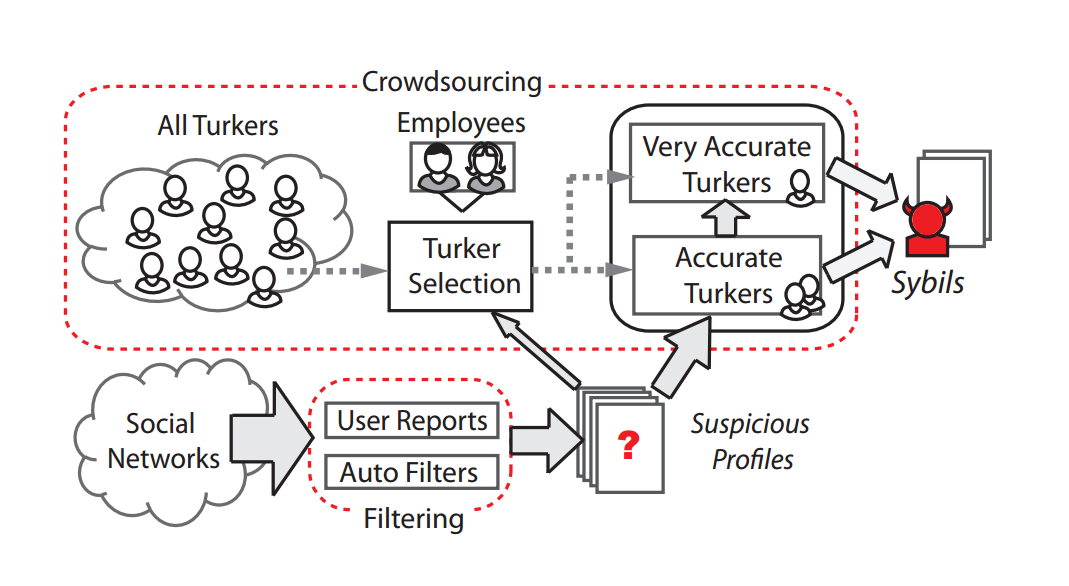
\includegraphics[scale=0.4]{fig/crowdsys}
	\caption{A crowd-sourced sybil detection system introduced by Wang et al. \cite{wangcrowd}.}
	\label{crowdsys}
\end{figure}

The system is working like this: The social network respectively social media platform that is to be defended generates suspicious profiles. This can either happen through explicit reports from users or through automatically applied filters that detect abnormal behavior. The so obtained profiles are then checked by crowd-sourced workers, which are subdivided in accurate and very accurate. To establish this differentiation, some of the suspicious profiles are mixed with some profiles that are known to be sybils. They are presented to all workers and their results allow a classification and to filter out unreliable workers. In the actual checking process, the profiles are first presented to the accurate workers which make a majority vote. If their decision is not clear, the profiles are presented to the very accurate workers which once again make a majority vote. 
The authors claim, that a system like this is very reliable and cost effective. 

Though such a social bot detection approach based on crowd-sourcing seems very promising at first sight, several problems become obvious on closer examination. First of all, this approach works optimal if every newly created profile can be reviewed in the above described way. However, young social media platforms will probably not be able or willing to pay for this bot detection scheme. A factor that may influence this could be also, that those platforms probably do not have huge issues with the social bot problem in their early stages. Once the platform has grown an the issue arises though, their is usually already a huge user base that has to be reviewed retrospectively. This is not optimal and may take a considerable amount of time.

Another point that mus be taken into consideration is that this approach might not be suitable for all types of social media platforms. While it might be well suited for platforms like Facebook or Renren, where profile pages can be customized a lot and contain usually plenty of information, other networks, like for example Twitter could be less appropriate. Generally it can be said that this detection approach is highly based on the information given in the users' profiles. If the information contained in the profiles is low, human investigators will probably not be able to distinguish as precisely as in the tests of Wang et al.

The last and probably most difficult issue that has to be mentioned is connected to this. Human investigators that are charged with distinguishing between bots and legitimate users have to have access to the profiles of the users. While those profiles are sometimes publicly available anyways, detailed profiles, which are more interesting for this approach, are, as discussed above, usually only visible for certain users. It is not hard to see the privacy issue that arises here, especially when keeping in mind, that the investigators are -- at least to a great extent -- only crowd-sourced workers, that can not be supervised as easily as ordinary employees \cite{ferrara15}.


\subsection{Based on Features}
The last detection approach for social bots is based on features. Features hereby means observable characteristics of posted information, profiles and possibly everything else that can be associated to the account in question. Schemes that make use of this approach often also use machine learning algorithms. That are algorithms that are able to make decisions based on learned patterns. They basically consist of two phases. In the first phase, the so called training phase, the algorithm processes training data which is labeled with the decision that should be made on this piece of data. By processing a lot of training data, the algorithm learns the features that are indicators for a certain decision. In the second phase, real data is processed and the algorithm is able to make decisions based on the learned data. Thus, schemes that make use of this detection approach can be compared to anomaly based intrusion detection systems. In the social bot detection topic, the decision being made is usually whether a specific account is controlled by a bot or a human. Since it is not easy to make a clear decision in many cases, there are often multiple decision options that each express a degree of certainty.

A well known example for this kind of social bot detection is the Bot or Not? system, presented by Davis et al. in \cite{botornot}. It is a publicly available\footnote{http://truthy.indiana.edu/botornot} system that allows a feature based social bot detection for accounts on the social media platform Twitter. Bot or Not? was trained with about 31.000 account samples of both, human and social bot accounts. For classification makes use of more than 1.000 features that can be assigned to six feature-classes. In the following we want to mention these classes shortly:
\begin{itemize}
	\item \textbf{Network} features reflect on the spreading of information, for example citations of different users or the like.
	\item \textbf{User} features take the information given in the actual account into consideration. Meta-data, that is basically data about data, is especially relevant in this feature. 
	\item \textbf{Friends} features are about the social relationships the account in question has.
	\item \textbf{Temporal} features analyze issues like the rate in which content is produced and the like.
	\item \textbf{Content} features are about wording characteristics in the texts produced by the relevant account.
	\item \textbf{Sentiment} features reflect on emotional aspects and are obtained by using specific algorithms \cite{botornot}.
\end{itemize}  
If a Twitter account name is entered in the Bot or Not? system, it checks all of those features and afterwards decides, based on the former mentioned training data, whether this account is a human or bot account.

Another social bot detection approach that can be classified as, kind of, feature based relies on detecting the coordinated behavior between social bots. Schemes that make use of this approach focus generally on the above described network, content and temporal features and often incorporate some graph theory as well. They usually aim at detecting attacks which try to distract from unpleasant facts or to distribute fake facts, like in the above described astroturf attack.  An example for such a scheme is SynchroTrap, presented by Cao et al. in \cite{synchrotrap}. Again, comparable to anomaly based intrusion detection systems, SynchroTrap makes use of clustering algorithms. These algorithms try to group values, that are similar in some aspects into distinct sets. 

The system monitors all user activity on a social media platform over an extended time period and monitors aggregated user actions. Then, the pairwise similarity between actions is determined and a hierarchical clustering algorithm is used to group users that show similar behavior at approximately the same time. If a cluster is growing too big, it can be assumed as malicious, since legitimate users tend to behave diverse \cite{synchrotrap}.

An issue with this detection method is though, that it is for example not able to detect bot accounts that show a mixture of bot and human behavior. Thus, the detection systems have to be developed further in order to keep up with the fast evolving social bots and their evermore sophisticated behavior \cite{ferrara15}.


\section{Summary and Outlook}
In the last chapter, we firstly introduced the term social bot, defined it and looked at the history of robots in social media.  Afterwards we gave a really short overview about Twitter, Facebook and Renren and motivated why social bot detection is important after all. In the main part of this chapter we discussed social bot detection approaches. We distinguished hereby social network information based, crowd-sourcing based and feature based approaches. 

Social network based approaches model the analyzed OSN into a graph where users correspond to the vertices and relationships between the users correspond to the edges of the graph. Afterwards, an algorithm tries to make a decision whether a given node is a social bot or an actual user. The decision is hereby usually based on the connections the node and his surroundings have. As examples for this kind of detection approach, we mentioned SybilGuard\cite{sybilguard}, SbilyInfer\cite{sybilinfer}, SumUp\cite{sumup} and the Facebook Immune System\cite{fis}. A problem these systems have to cope with is, that they tend to assume, that bots can't establish relationships to actual, what emerged to be not true.

Next we elaborated on crow-sourcing based approaches. The basic underlying idea of these approaches is to engage actual humans to analyze given user profiles and to decide whether those belong to an actual user or a social bot. We discussed the paper "Social turing tests: Crowdsourcing sybil detection" by Wang et al. \cite{wangcrowd} which analyzes this approach thoroughly and introduces a general practical system. One of the issues this approach has to handle is that some social networks users don't have very detailed profiles what makes crowd-sourced bot detection very hard. 

At last, we discussed feature based social bot detection approaches. They observe characteristics of OSN users and information published by them in order to decide -- or give a tendency -- whether a given account is a bot, or not. Often, they make use of machine learning algorithms. This means that, in a first step, they are trained with datasets in which it is known whether a profile is bot- or human-owned. Afterwards they are used to make decisions about real data. As an example we introduced the Bot or Not? system by Davis et al. \cite{botornot}.

After analyzing the different detection approaches, it becomes apparent that a combination of different approaches yield good results. Observing the social graph and behavioral features of accounts together is for example a promising strategy. Ferrara et al. bring in the Renren sybil detector \cite{wang2013, yang2014} as a good example for these combined approaches \cite{ferrara15}.

However, it has to be noted that not all robots in social media have to be necessarily evil. Some social bots provide useful services that many users don't want to miss. It is just important, that users are able to distinguish between other humans and bots for example in order to differentiate whether content they see is actually as popular as it seems.

It is safe to assume that the number of social bots will increase even more and that their methods and behaviors will get even more sophisticated. We expect an arms race between bot herders and bot detection mechanisms, like it was -- and still is -- the case with malware and malware detection software.

























\newpage